\chapter{Periodo Orbital} \label{metodologia:analisisperiodo}

Una de las propiedades más importantes presente en la curva de luz de una
binaria eclipsante es su \textit{periodo orbital}. Partiendo del periodo orbital
es posible presentar los datos observacionales en el espacio fase en vez de
tiempo, el cual nos permite ajustar un modelo cuyos parámetros expliquen una
característica física del sistema. Dada una curva de luz se puede encontrar el
periodo orbital usando \textbf{periodogramas}: herramientas utilizadas para
generar un espectro de potencias para una serie de tiempo periódica. Para series
de tiempo cuyo muestreo no es uniforme en el tiempo (como es común de
observaciones astronómicas) se utiliza el periodograma \textbf{Lomb-Scargle},
derivado de la transformada de Fourier y descrito por
\citeyearparen{vanderplas_understanding_lomb_scargle_periodogram_2018}. En
particular se utiliza una generalización del periodograma Lomb-Scargle que se
utiliza para ajustar curvas de luz en diferentes bandas al mismo tiempo; el
periodograma de \textit{Lomb-Scargle multibanda} utiliza un modelo de Fourier
truncado que describe la variabilidad en común de todas las bandas en las que se
observó el sistema, y a este le suma un modelo de ajustes de Fourier truncados
para cada banda individual, el cual ajusta la variabilidad vista en los residuos
del ajuste del término en común
[\citeyearparen{vanderplas_periodograms_lombscargle_multiband_2015}]. Usando un
mallado suficientemente fino para explorar el espacio de frecuencias se puede
encontrar la frecuencia de mayor potencia, indicando el periodo orbital del
sistema; al mismo tiempo, para restringir esta malla de periodos se impuso un
límite máximo de 1 día, basado en las primeras observaciones de Iturbide. El
espectro de frecuencias se encuentra en la \reffigure{periodogramaLSFrecs}. 

\begin{figure}[!ht]
	\centering
	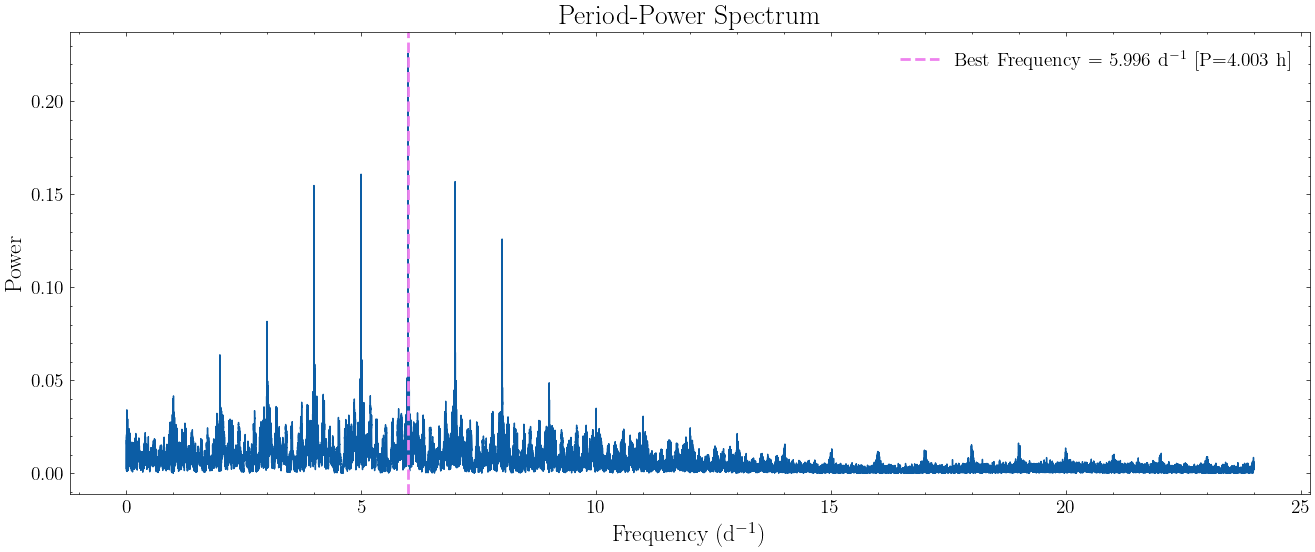
\includegraphics[scale=0.45]{Metodologia/Secciones/AnalisisPeriodo/Figures/LS Power Spectrum.png}
	
	\caption{Espectro de frecuencias de las curvas de luz fotométricas de
	\atoObjIdNoSpace, utilizando todas las observaciones recabadas de Gaia, ZTF,
	e Iturbide. El pico de más alta potencia está ubicado en el periodo de
	aproximadamente $0.1668 \ \mathrm{d} \ (4.003 \ \mathrm{h})$.} 
	\label{periodogramaLSFrecs}
\end{figure}

Dado este espectro de frecuencias encontramos que el periodo orbital es igual a
la frecuencia principal multiplicada por 2. Esto se debe a los requisitos para
analizar una curva de luz de un sistema binario eclipsante, los cuales muestran
dos valles en el espacio fase, cada uno correspondiendo a los eclipses de la
componente primaria y la secundaria respectivamente. La curva de luz en fase la
cual muestra ambos eclipses se puede ver en la
\reffigure{gaiaIturbideZtfPhaseFold}. El periodo orbital encontrado es de
8.005584950787622 horas. Se hizo uso de la implementación del periodograma
Lomb-Scargle para multiples bandas de \code{astropy}, utilizando la clase
\href{https://docs.astropy.org/en/stable/timeseries/lombscarglemb.html}{\code{LombScargleMultiband}}.
El código donde se realizó el análisis se encuentra en el Notebook
\href{https://github.com/KnightIV/UANL_MAPTA_Observaciones/blob/main/analisis/period-analysis/periodogram.ipynb}{\code{periodogram.ipynb}}.

\begin{figure}[!h]
	\centering
	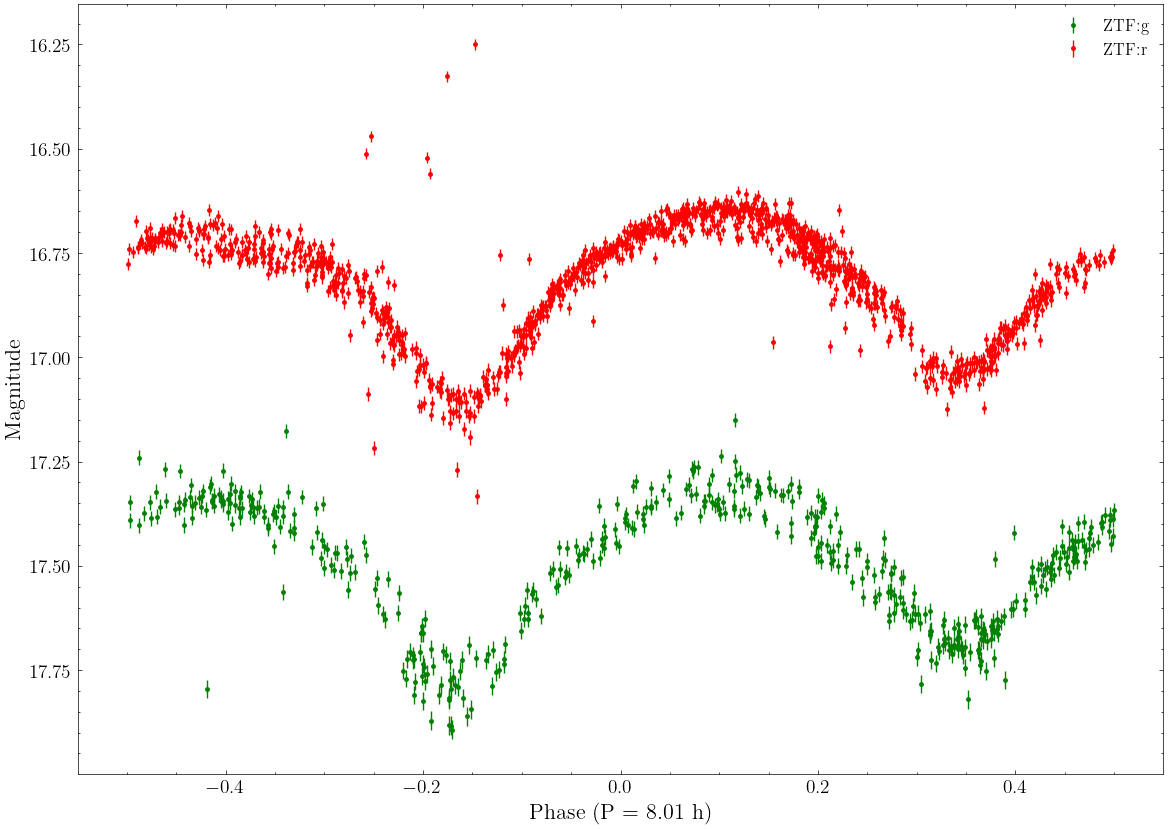
\includegraphics[scale=0.28]{Metodologia/Secciones/AnalisisPeriodo/Figures/ZTF Phase-Folded.png}
	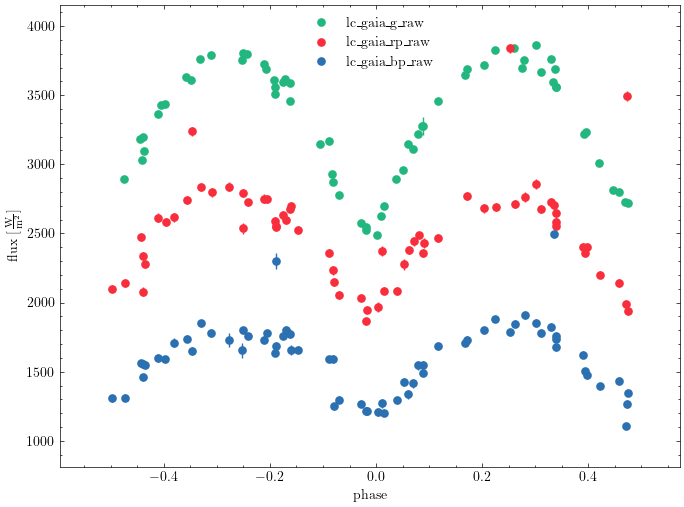
\includegraphics[scale=0.28]{Metodologia/Secciones/AnalisisPeriodo/Figures/Gaia Phase-Folded.png}
	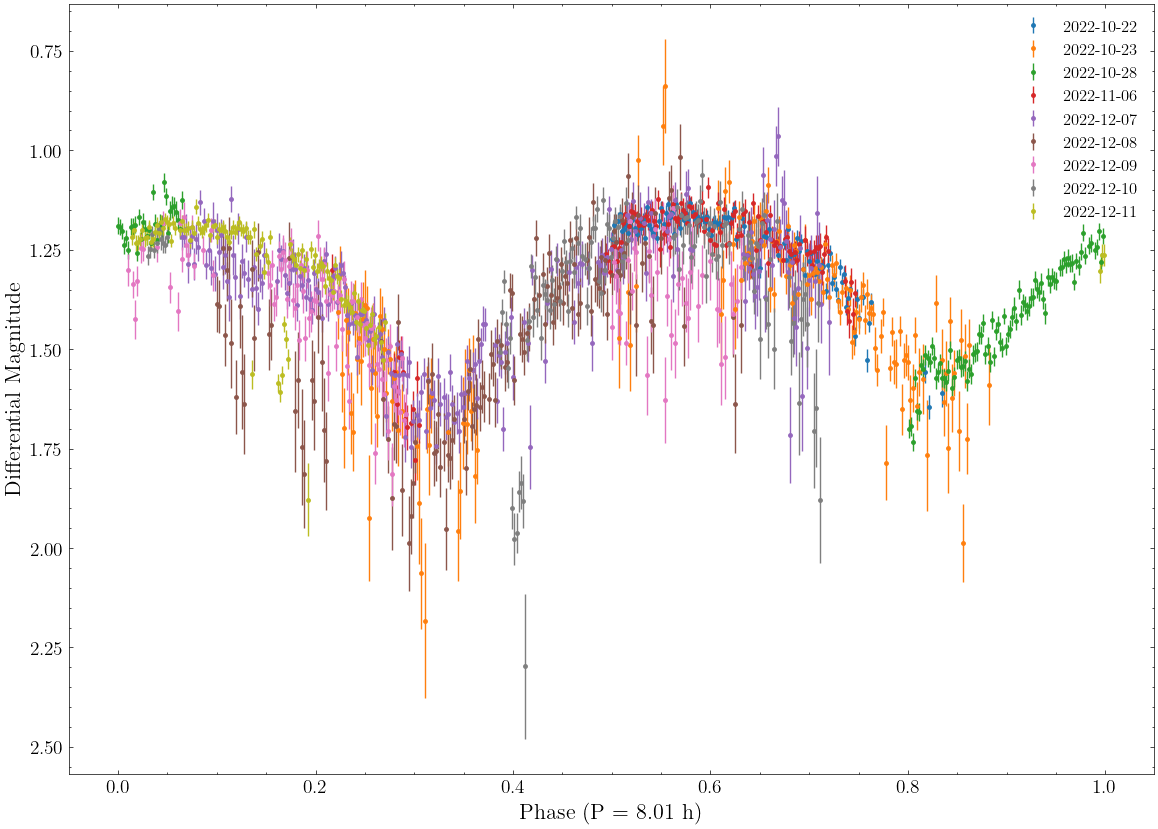
\includegraphics[scale=0.37]{Metodologia/Secciones/AnalisisPeriodo/Figures/Iturbide Phase-Folded.png}

	\caption{Curvas de luz de ZTF, Gaia e Iturbide en espacio fase dado un
		periodo orbital de 8.005584950787622 horas. El tiempo de conjunción
		superior son corregidos en los siguientes pasos de afinación del modelo
		de PHOEBE, el cual ajusta la fase 0 para que coincidan las 3 curvas de
		luz. Las observaciones de Iturbide se clasifican por su noche de
		observación, indicado por su color.}
	\label{gaiaIturbideZtfPhaseFold}
\end{figure}